%% LyX 2.0.7 created this file.  For more info, see http://www.lyx.org/.
%% Do not edit unless you really know what you are doing.
\documentclass[letterpaper,english]{scrartcl}
\usepackage{fourier}
\usepackage{verbatim}
\usepackage{helvet}
\usepackage[OT2,T1]{fontenc}
\usepackage{color}
\definecolor{shadecolor}{rgb}{0.75, 0.75, 0.75}

\DeclareSymbolFont{cyrletters}{OT2}{wncyr}{m}{n}
\DeclareMathSymbol{\Sha}{\mathalpha}{cyrletters}{"58}
\usepackage[T1]{fontenc}
\usepackage[latin9]{inputenc}
\pagestyle{empty}
\setlength{\parskip}{\smallskipamount}
\setlength{\parindent}{0pt}
\usepackage{babel}
\usepackage{placeins}
\usepackage{multicol}
\usepackage{units}
\usepackage{amsmath}
\usepackage{graphicx}
\usepackage{setspace}
\usepackage{esint}

\usepackage[T1]{fontenc}
\usepackage[latin9]{inputenc}
\pagestyle{empty}
\setlength{\parskip}{\smallskipamount}
\setlength{\parindent}{0pt}
\usepackage{color}
\definecolor{shadecolor}{rgb}{0.75, 0.75, 0.75}
\usepackage{babel}
\usepackage{units}
\usepackage{framed}
\usepackage{amsmath}
\usepackage{amssymb}
\usepackage{graphicx}
\usepackage{setspace}
\usepackage{esint}

\onehalfspacing
\usepackage[unicode=true,
 bookmarks=true,bookmarksnumbered=false,bookmarksopen=false,
 breaklinks=false,pdfborder={0 0 1},backref=false,colorlinks=false]
 {hyperref}
\hypersetup{pdftitle={Physics 175 - Problem Set 1},
 pdfauthor={Anton Mazurenko}}

\makeatletter

%%%%%%%%%%%%%%%%%%%%%%%%%%%%%% LyX specific LaTeX commands.
\pdfpageheight\paperheight
\pdfpagewidth\paperwidth

\newcommand{\noun}[1]{\textsc{#1}}
%% Because html converters don't know tabularnewline
\providecommand{\tabularnewline}{\\}

%%%%%%%%%%%%%%%%%%%%%%%%%%%%%% User specified LaTeX commands.
\usepackage{scrpage2}
\usepackage{xcolor}


%%LaTeX for Physicists
\let\vaccent=\v % rename builtin command \v{} to \vaccent{}x
\renewcommand{\v}[1]{\ensuremath{\mathbf{#1}}} % for vectors
\newcommand{\gv}[1]{\ensuremath{\mbox{\boldmath$ #1 $}}} 
% for vectors of Greek letters
\newcommand{\uv}[1]{\ensuremath{\mathbf{\hat{#1}}}} % for unit vector
\newcommand{\abs}[1]{\left| #1 \right|} % for absolute value
\newcommand{\avg}[1]{\left< #1 \right>} % for average
\let\underdot=\d % rename builtin command \d{} to \underdot{}
\renewcommand{\d}[2]{\frac{d #1}{d #2}} % for derivatives
\newcommand{\dd}[2]{\frac{d^2 #1}{d #2^2}} % for double derivatives
\newcommand{\pd}[2]{\frac{\partial #1}{\partial #2}} 
% for partial derivatives
\newcommand{\pdd}[2]{\frac{\partial^2 #1}{\partial #2^2}} 
% for double partial derivatives
\newcommand{\pdc}[3]{\left( \frac{\partial #1}{\partial #2}
 \right)_{#3}} % for thermodynamic partial derivatives
\newcommand{\ket}[1]{\left| #1 \right>} % for Dirac bras
\newcommand{\bra}[1]{\left< #1 \right|} % for Dirac kets

\newcommand{\braket}[2]{\left< #1 \vphantom{#2} \right|
 \left. #2 \vphantom{#1} \right>} % for Dirac brackets

\newcommand{\matrixel}[3]{\left< #1 \vphantom{#2#3} \right|
 #2 \left| #3 \vphantom{#1#2} \right>} % for Dirac matrix elements
\newcommand{\grad}[1]{\gv{\nabla} #1} % for gradient
\let\divsymb=\div % rename builtin command \div to \divsymb
\renewcommand{\div}[1]{\gv{\nabla} \allcdot #1} % for divergence

\newcommand{\Ham}{\mathcal{H}} %for Hamiltoninan
\newcommand{\emf}{\mathcal{E}} %E field
\newcommand{\dpl}[1]{\mathcal{P}_{#1}}
\newcommand{\conj}[1]{\overline{#1}}

\newcommand{\curl}[1]{\gv{\nabla} \times #1} % for curl
\let\baraccent=\= % rename builtin command \= to \baraccent
\renewcommand{\=}[1]{\stackrel{#1}{=}} % for putting numbers above =




\ihead{\LARGE\bfseries Physics 175}
\ohead{\LARGE Practice Mid-Term Exam}
\setheadsepline{.8pt}
\setkomafont{pagehead}{\sffamily}
\setkomafont{headsepline}{\color{black!50}}
\pagestyle{scrheadings}

\usepackage{titlesec}
\titleformat{\subsection}[hang]
       {\normalfont\bfseries}
       {(\alph{subsection})}
       {0.5em}
       {}
       []
\titleformat{\paragraph}[hang]
       {\normalfont\bfseries}
       {}
       {0.5em}
       {}
       []

\makeatother

\begin{document}

\title{Practice Mid-Term Examination}

\subtitle{Physics 175}

\date{March 21/23, 2017}

\maketitle

\section*{Name: \rule{0.5\columnwidth}{1pt}}

\section*{Instructions}

You will have 90 minutes to work on the exam. The exam is a total of 100 points. There are 6 problems
totaling 96 points.Turning in your formula sheet is worth the remaining 4 points.  Budget your time wisely, using the point values
as a guide. Use empty pages for computation.

An equation sheet containing all required equations (and then some!) can be found in the back.

You are not allowed to use any material (books, lecture notes) other
than \emph{double-sided sheet with your handwritten notes}, which
you're required to hand in together with your exam. The use of a calculator
is permitted, but no other electronic device (cell phone, laptops,
etc.) are allowed during the exam.

Extra paper is available should you require it. Please write your
name on \emph{every} sheet that you attach to your exam.

\begin{table}[ht]
\centering
\begin{tabular}{cc}
\textbf{Problem} & \textbf{Score}\\[0.5ex]
1 & \rule{20pt}{1pt}\\ [0.5ex]
2 & \rule{20pt}{1pt}\\[0.5ex]
3 & \rule{20pt}{1pt}\\[0.5ex]
4 & \rule{20pt}{1pt}\\[0.5ex]
5 & \rule{20pt}{1pt}\\[0.5ex]
\textbf{TOTAL} & \rule{20pt}{1pt}\\

\end{tabular}
\end{table}

\noindent \begin{center}
\noun{Good Luck}!
\par\end{center}

\clearpage{}



\section{Lenses}


\subsection{Lens Equations}

\begin{shaded}
What is the lens equation?
\end{shaded}

\[ 
\frac{1}{f}=\frac{1}{s_i}+\frac{1}{s_o}
\]

\subsection{Imaging: Conceptual}
\begin{shaded}
What is the focal length of a lens?

\emph{Answer this in words or using the lens equation}
\end{shaded}


There are two common answers for this:
\begin{enumerate}
\item The $2f\rightarrow 2f$ problem below is one common way. This defines the $f$ as the length that images an object at a distance in front of the lens to the same length behind the lens.
\item Another common answer is that parallel waves, or objects at infinity, are imaged to the focal length away from the lens.  This can be described vice versa as well.
\end{enumerate}

\subsection{Imaging}
\begin{shaded}
Where is an object imaged to if it is placed $z_o=2f$ in front of the lens at $z=0$?
\end{shaded}

\[
\frac{1}{f}=\frac{1}{2f}+\frac{1}{z}
\]
\[
z\rightarrow 2f
\]

\section{Fourier Transforms}

\subsection{Important Examples}

\begin{shaded}
What is the fourier transform of f(x)?
\[
f(x)=\delta (x-x_o)+\delta (x+x_o)
\]
\end{shaded}


\[
F(x)=\mathcal{F}[f(x)]=\frac{2}{\sqrt{2 \pi}} \cos{k_x x_o}
\]




\begin{shaded}
What is the fourier transform of f(x)?
\[
f(x)=\sin{k_x x_o}
\]
\end{shaded}


\[
F(x)=\mathcal{F}[f(x)]=\frac{\sqrt{2 \pi}}{2 i} \left ( \delta (x+x_o)-\delta (x+x_o) \right )
\]

\subsection{4F Systems}

\begin{shaded}
What mathematical function do lenses perform?
\end{shaded}

They perform fourier transforms from $z=-f$ to $z=f$!

\begin{shaded}
\subsection{4F imaging}

Consider a 4F imaging system where a gaussian beam, with flat phase front at $z=-f_1$ is imaged by a lens with focal length $f_1$ to a plane $z=f_1$ where it impinges on an ideal grating  with spacing $d$.

The electric field at $z=-f_1$ is given below:
\[
E(z=-f_1)=G_{0,\sigma}(x)
\]

The mask function $M(x')$, ideal grating in this case, is given functionally below:
\[
M(x)=\Sha_d(x)=\sum_{n=-\infty}^{\infty}\delta(x-nd)
\]

\emph{Refer to equation sheet at end of test if confused about these functions}
\end{shaded}

\begin{figure}[h!]
\begin{center}
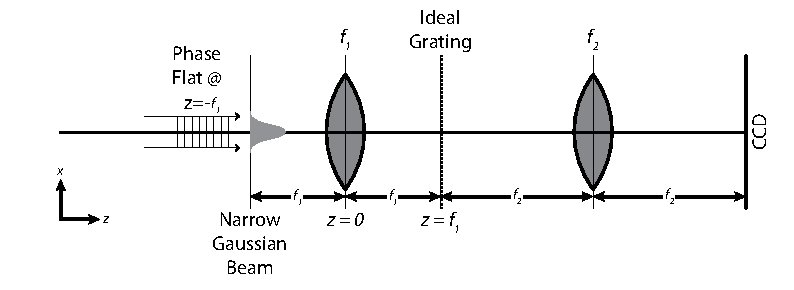
\includegraphics[scale=0.95]{ph175_4f_mod}
\caption{4F imaging system. Problem \textbf{2a}}
\end{center}
\end{figure}

\begin{shaded}
\begin{enumerate}
\item Write on the figure where the ``Fourier Plane" is for this imaging system.
\item Determine what the electric field is  (as a function of $k_x$) just before hitting the ideal grating/mask at $z=f_1 - \epsilon$, ($\epsilon\ll f_1$).
\item Rewrite the electric field as a function of transverse coordinate $x'$ at $z=f_1 - \epsilon$, ($\epsilon\ll f_1$).
\item Determine the electric field just after illuminating the ideal grating,$M(x')$, as a function of transverse coordinate $x'$ at $z=f_1 + \epsilon$, ($\epsilon\ll f_1$).
\item Determine the electric field now at the CCD chip ($z=f_1+2f_2$). (For simplicity of the solution, assume that $2\pi/d\gg \sigma$.
\end{enumerate}

\emph{Hint:} Remember that when changing from $k$-space to real dimensions we use the substitution $k_x\rightarrow \frac{2 \pi}{\lambda f} x'$. 

\emph{Hint:} The scaling theorem and convolution theorem may be \emph{very} useful in this problem.
\end{shaded}

\begin{enumerate}
\item The fourier plane is exactly where the ``Ideal Grating" is located.

\item We can refer to the formula sheet at the end of the midterm where we can pull out the Gaussian fourier transform formula out.
Which will give us the Gaussian just before the ideal grating.
\[
\mathcal{F}\left [ G_{0,\sigma}(x) \right ]= G_{0,1/\sigma}(k_x)
\]

\item Using the hint, we can rewrite the formula above to:
\[
\sigma G_{0,1/\sigma} \left ( \frac{2 \pi }{\lambda f_1}x' \right )
\]

\item The electric field after the grating will just be the multiplication of the grating and the Gaussian beam.
\[
G_{0,1/\sigma} \left ( \frac{2 \pi }{\lambda f_1}x' \right ) \sum_{n=-\infty}^{\infty}\delta(x'-nd)  
\]

\item Using the convolution theorem and the scaling theorem (also our knowledge about 4f systems) we can realize that at the CCD the answer is of the form
\[
\mathcal{F} \left [ \sum_{n=-\infty}^{\infty}\delta(x'-nd)   \right  ] \ast \mathcal{F} \left  [\sigma G_{0,1/\sigma} \left ( \frac{2 \pi }{\lambda f_1}x' \right ) \right ]
\]

Be careful here to use the scaling theorem of the fourier transform to end up getting the magnification inside the gaussian correct!

\[
\left [ \frac{\sqrt{2 \pi} }{d} \Sha_{2 \pi /d} \left ( \frac{2 \pi }{\lambda f_2}x' \right ) \right ] \ast \left [\frac{f_1 \lambda}{2 \pi} G_{0,\sigma}  \left ( \frac{f_2}{f_1} x' \right ) \right ]
\]

With the assumption that $\sigma\ll d$, then this answers is approximately

\[
\approx  \sum_{n=-\infty}^{\infty}  G_{0,\sigma}  \left ( \frac{2 \pi }{\lambda f_2} \left  ( x' - n \frac{2 \pi}{d} \right ) \frac{f_2}{f_1} \right )
\]

\end{enumerate}

\newpage
\clearpage{}
\newpage

\section{Filters by eye}


\subsection{Filters}

\begin{shaded}
For the following image, guess which resultant image is a function of the input image (top left) and the fourier filter (top right)
\end{shaded}

\begin{figure}[h!]
\begin{center}
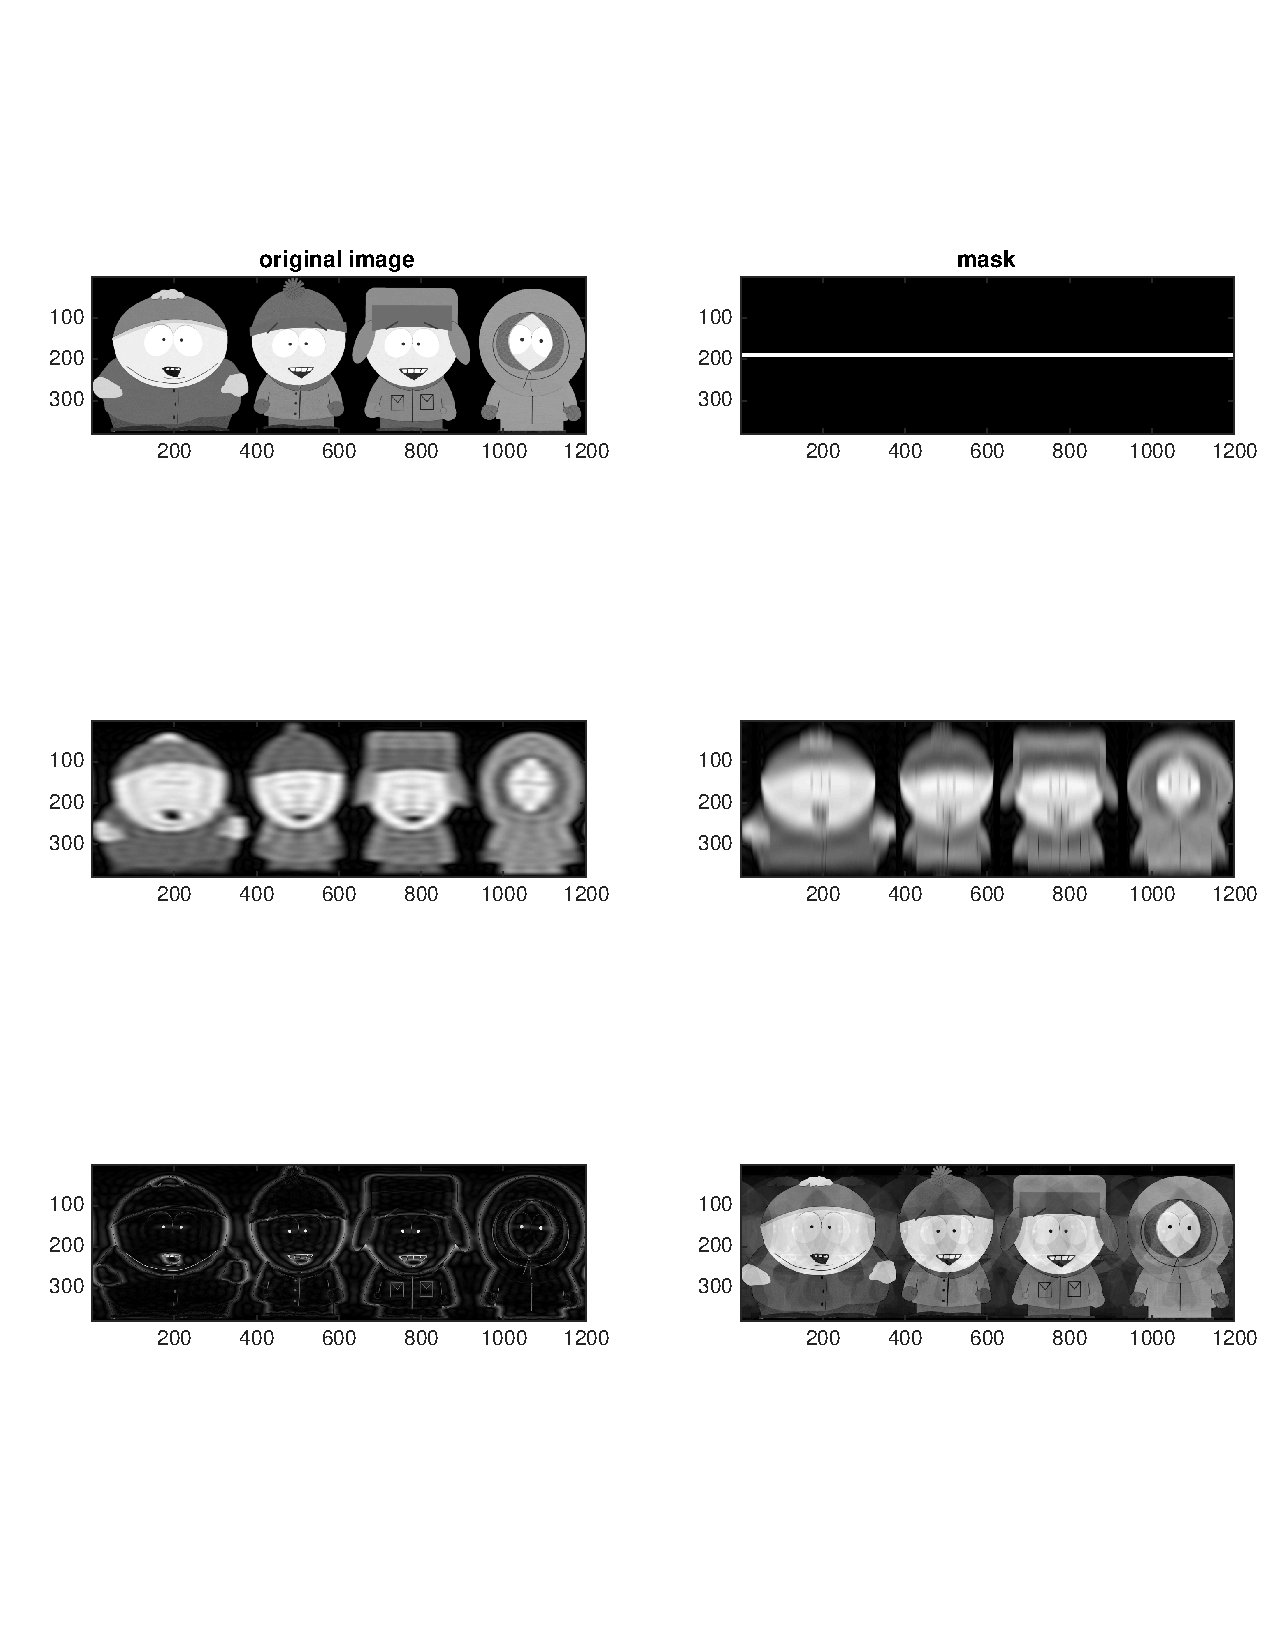
\includegraphics[scale=0.4]{fft_figs/pp1.pdf}
\caption{4F imaging system with filtering. Top Left is the original image. The Filter in the fourier plane is the top right image.}
\end{center}
\end{figure}

\newpage

\begin{shaded}
For the following image, guess which resultant image is a function of the input image (top left) and the fourier filter (top right)
\end{shaded}

\begin{figure}[h!]
\begin{center}
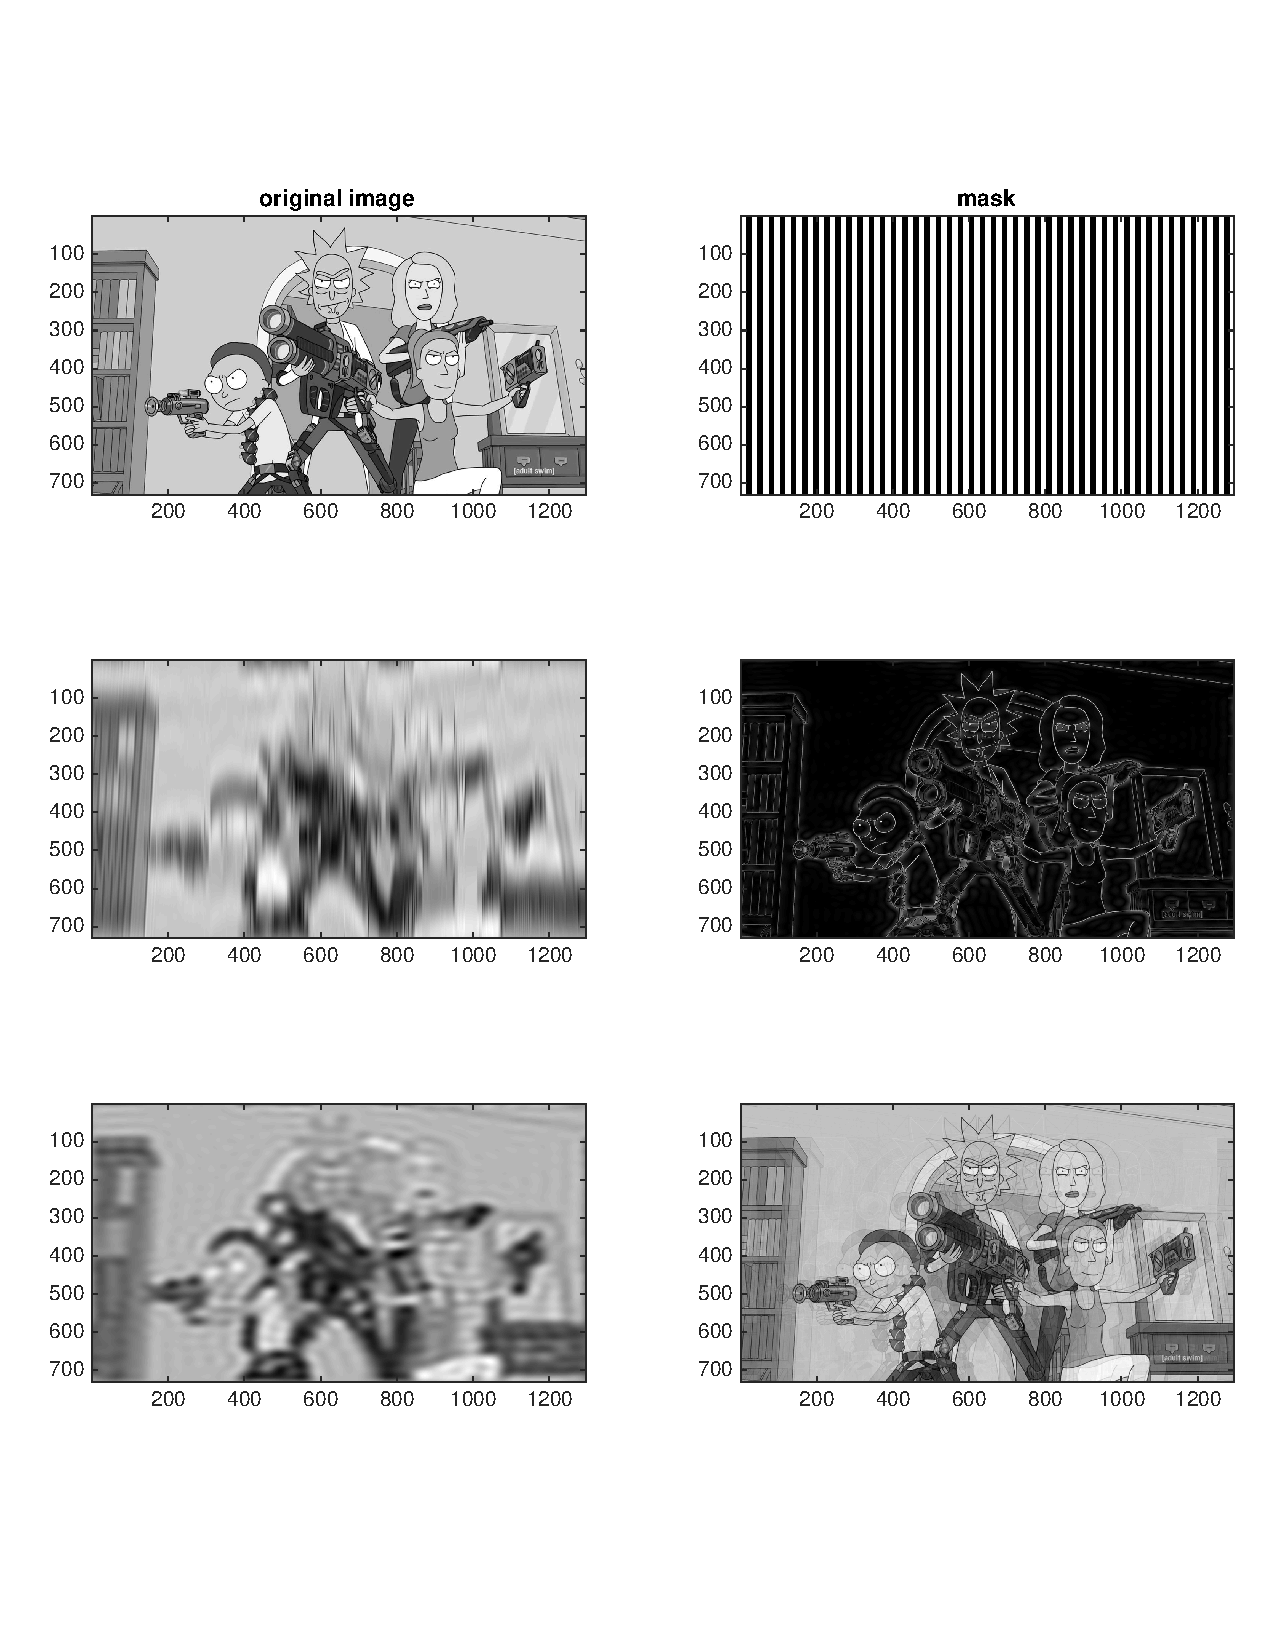
\includegraphics[scale=0.5]{fft_figs/pp2.pdf}
\caption{4F imaging system with filtering. Top Left is the original image. The Filter in the fourier plane is the top right image.}
\end{center}
\end{figure}

\newpage
\begin{shaded}
For the following image, guess which resultant image is a function of the input image (top left) and the fourier filter (top right)
\end{shaded}

\begin{figure}[h!]
\begin{center}
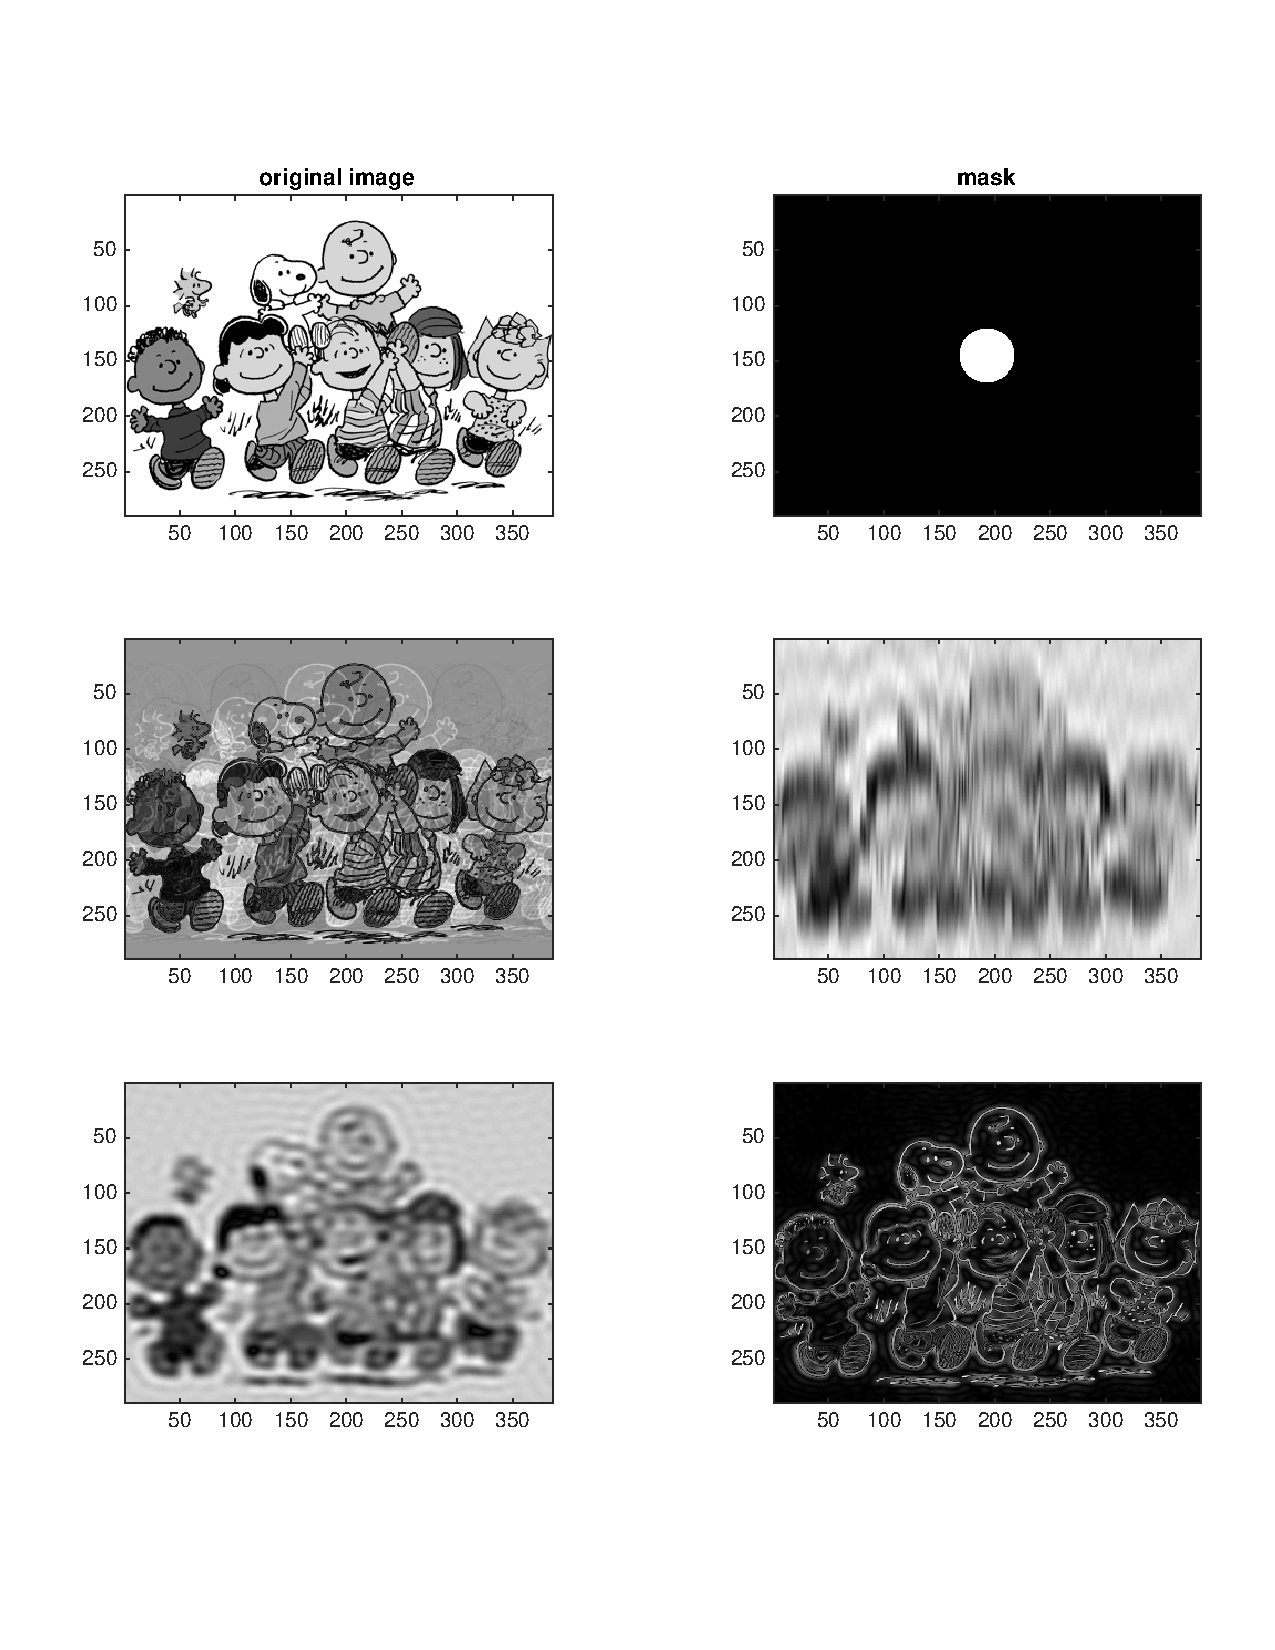
\includegraphics[scale=0.5]{fft_figs/pp3.pdf}
\caption{4F imaging system with filtering. Top Left is the original image. The Filter in the fourier plane is the top right image.}
\end{center}
\end{figure}

\newpage
\begin{shaded}
For the following image, guess which resultant image is a function of the input image (top left) and the fourier filter (top right)
\end{shaded}

\begin{figure}[h!]
\begin{center}
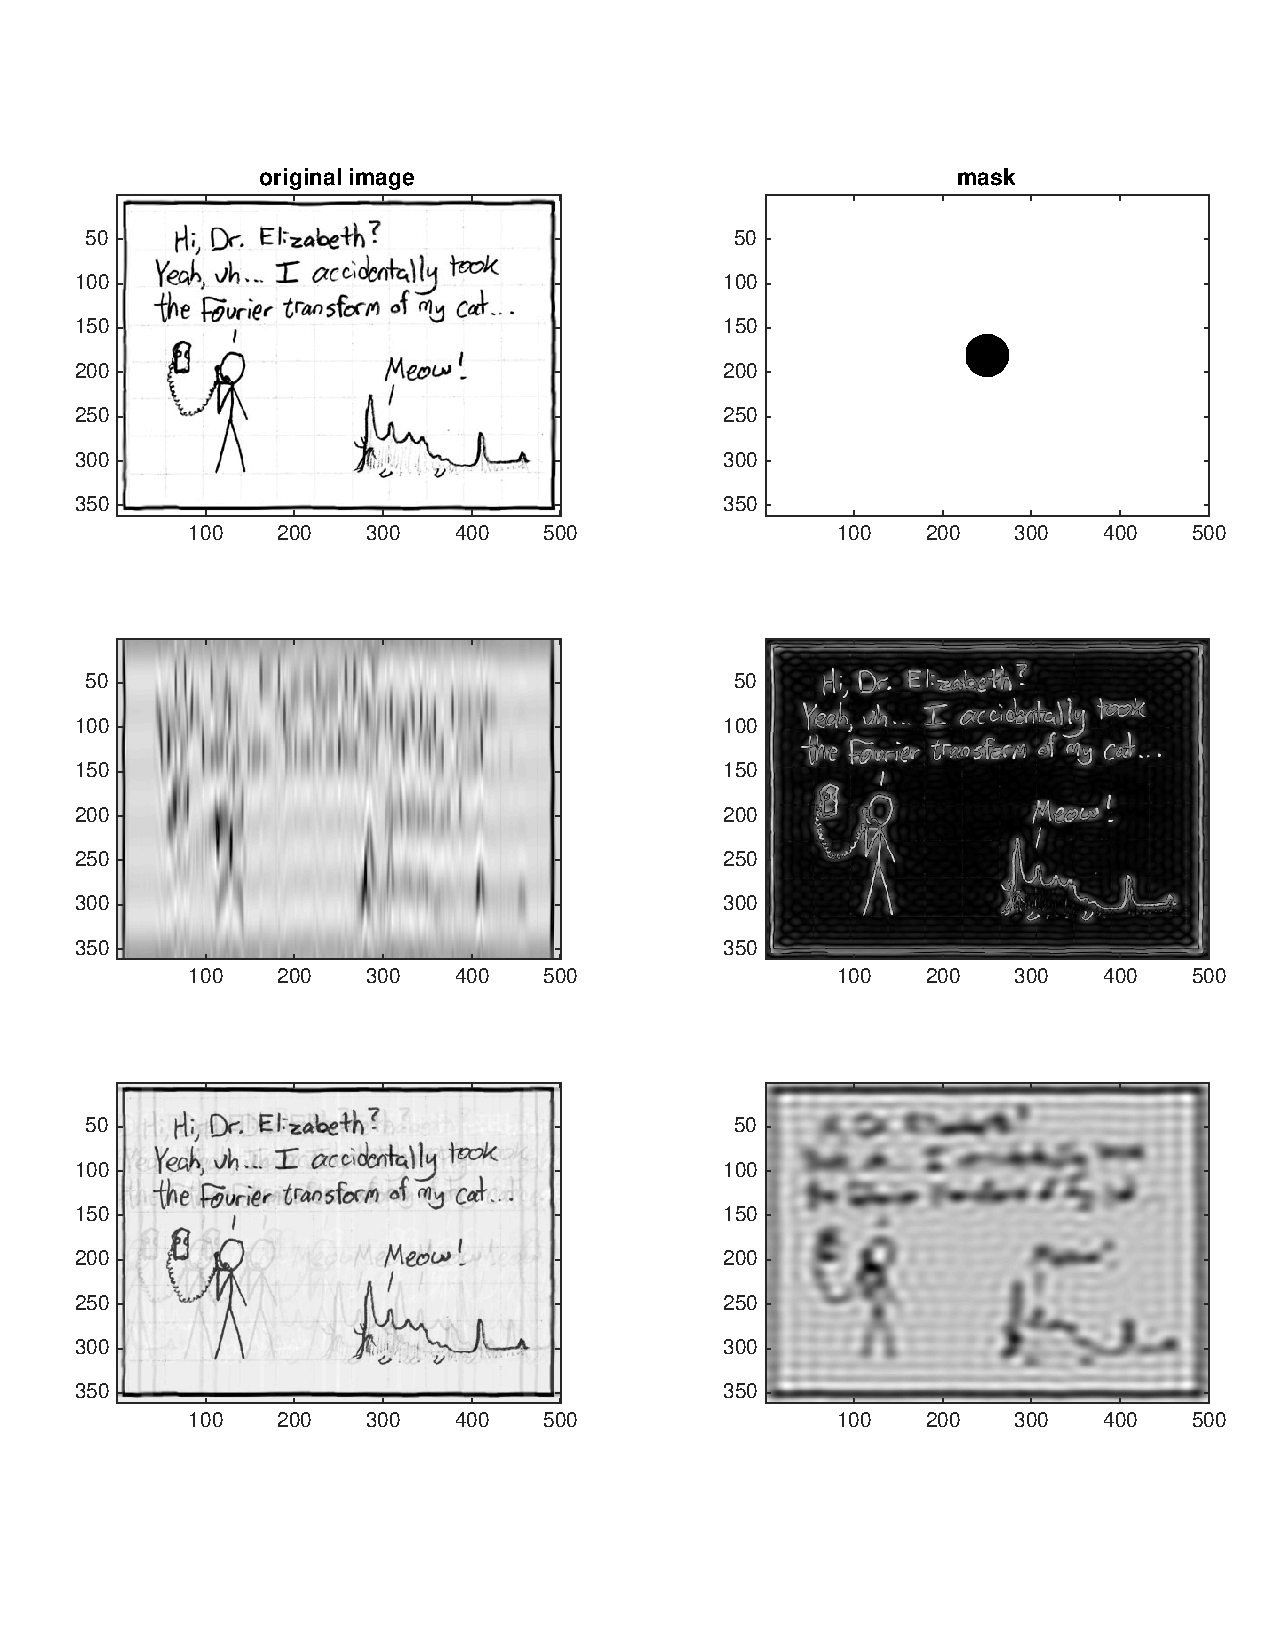
\includegraphics[scale=0.5]{fft_figs/pp4.pdf}
\caption{4F imaging system with filtering. Top Left is the original image. The Filter in the fourier plane is the top right image.}
\end{center}
\end{figure}

\newpage

\subsection{Answers}
\begin{itemize}
\item middle right picture
\item bottom right picture
\item bottom left picture
\item middle right picture
\end{itemize}

\clearpage{}
\newpage


\section{Gaussian Modes}

\subsection{Qualitative Question 1}
\begin{shaded}
What equation does the ``Gaussian Beam" satisfy?
\end{shaded}

Paraxial Helmholtz Equation


\subsection{Qualitative Question 2}
\begin{shaded}
What is the ``rayleigh range" defined as?
\end{shaded}

So qualitatively (well, quantitatively too), it is defined as the places where the waist grows by a factor of $\sqrt{2}$ in amplitude.

As a definition it is a function of the minimum waist and the wavelength of the beam.

\emph{Remember:}
\[
z_o=\frac{\pi w_o^2}{\lambda}
\]

\subsection{Less Qualitative Question 3}
\begin{shaded}
If I want a waist of $w_o$, and I place a lens of $f$ at a location where the radius of curvature is infinite, and the beam has a waist of $w'$:
\begin{enumerate}
\item Where will the minimum waist be located?
\item What $f$ should the lens be?
\end{enumerate}
\end{shaded}


\emph{Remember:} The rayleigh range is determined from the minimum waist and $\lambda$.
\[
z_o=\frac{\pi w_o^2}{\lambda}
\]

\begin{enumerate}
\item 
The waist we start with and the waist we want detemrine the location of the minimum waist.
\[
w' = w_o \sqrt{1+\left ( \frac{z}{z_o} \right )^2}
\]

\[
\left ( \frac{w'^2}{w_o^2} - 1\right ) z_o^2 = z^2
\]

\item
\[
f=R(z)=z+\frac{z_o^2}{z}
\]
\end{enumerate}







\section{Cavities}

\begin{shaded}
Given a cavity with two mirrors of equal magnitude of curvature (the sign you can adjust based on placement) separated by $6 z_o$, what must the radius of curvatures be?
\begin{enumerate}
\item Consider the case where the mirrors are placed symmetrically on either side of the minimum waist.
\item Consider the case where the mirrors are placed both on one side of the minimum waist.
\end{enumerate}
\end{shaded}

\begin{enumerate}
\item The symmetric case is simple in the sense that the separation of $6 z_o$ also fixes the two mirrors to then be at $z=-3 z_o$ and $z=3 z_o$. 
Which then with the radius of curvature formula just gives us $R(z)=\frac{10}{3}z_o$ and $R(-z)=-\frac{10}{3}z_o$.

\item The case where the mirrors of are equal curvature and sign means they must be located both on one side of the waist. There is a maximum ``curviness" that the beam can have that is located exactly at the rayleigh range. So by placing mirrors on either side of the rayleigh range with same sign and curvature we can make a stable mode. Again, solve  the radius of curvature equation for one sign of $z$  where the two radius of curvatures are the same (just solve a quadratic equation of $R(z)$ for $z$). 


It's easier to use ``natural units" of $z_o$ for everything.
\[
R=z+\frac{z_o^2}{z}
\]
\[
0=z^2-Rz+z_o^2\rightarrow 0=\frac{z}{z_o}^2-\frac{R}{z_o} \frac{z}{z_o}+1
\]
So now absorb the $z_o$ into all the $z$ and $R$ factors
\[
z_{+,-}=\frac{R}{2}\pm\sqrt{\left ( \frac{R}{2} \right )^2-1}
\]

This will give a $z_+$ and a $z_-$. Then set the difference of these to the mirror separation of $6 z_o$.

\[
z_+-z_-=d=6 = 2 \sqrt{\left ( \frac{R}{2} \right )^2 -1}
\]

\[
36/4=\left ( \frac{R}{2} \right )^2 - 1 \rightarrow R=\sqrt{40}
\]

To get back into real units we can stick the $z_o$ back in.

$R=\sqrt{40}z_o$


\end{enumerate}




\section{Polarization}



\subsection{General Question 1}
\begin{shaded}
Using the Jones Vector notation, how do we find if another polarization is orthogonal?
\end{shaded}

Consider asking how we normalize an $\vec{E}$-field by dotting the complex conjugate of the field with itself.

\[
\vec{J^\dagger}\vec{J}=1
\]

So to find when they're orthogonal would mean that :
\[
\vec{J_i^\dagger}\vec{J_j}=0
\]

We know that for picking orthogonal vectors for purely real vectors we find the negative inverse of the vector. The only slight change we need to keep in mind is that for complex variables we have this conjugate transpose. So the conjugate transpose of the vector must be the negative inverse of the vector we have for it to be orthogonal.

Ex:
\[
J_1 \rightarrow \frac{1}{\sqrt{2}}
\left (
\begin{array}{c}
1\\
i \\ \end{array}
\right )
\]

So the orthogonal vector is:
\[
J_2 \rightarrow \frac{-1}{\sqrt{2}}
\left (
\begin{array}{c}
i\\
1 \\ \end{array}
\right )
\]

We can check this by taking the dot product of the two vectors
\[
J_1^\dagger J_2 = \frac{-1}{2} \left [ (-i)(1) + (i)(1) \right ] = 0
\]

\subsection{General Question}

\begin{shaded}
What does a $\lambda/2$ wave plate do? What are the ``fast" and ``slow" axes in the form of its matrix representation?
\end{shaded}

Looking at the formulat sheet is very enlightening.
Remember that a wave plate has birefringence such that one polarization sees a different index of refraction compared to another. This means that the effective path length for one polarization through the plate is also effectively different for each polarization! 
The ``fast" axis we typically describe as being the  one that gets no phase shift while the ``slow" axis is retarded or delayed compared to the ``fast" axis by a factor of $k_o\cdot d (\delta n)$.

This gives a differential phase of $exp(-i \phi)$ between the two axes where $\phi=k_o \cdot d (\delta n)$.

\subsection{Polarization Rotation}

\begin{shaded}
How can I rotate the polarization from 
\[
J_1 \rightarrow \frac{1}{\sqrt{2}}
\left (
\begin{array}{c}
1\\
0 \\ \end{array}
\right )
\rightarrow
J_2 \rightarrow \frac{1}{\sqrt{2}}
\left (
\begin{array}{c}
0\\
1 \\ \end{array}
\right )
\]

with a $\lambda/2$ wave plate?
\end{shaded}
 
Use the rotation matrices!

The matrix for the $\lambda/2$ plate is just given by : 
\[
\left (
\begin{array}{cc}
1 & 0 \\
0 & exp(i \phi) \\ \end{array}
\right )
\]

where $\phi=\pi$. Which gives:
\[
S_\pi=\left (
\begin{array}{cc}
1 & 0 \\
0 & -1 \\ \end{array}
\right )
\]

Transforming this matrix by the rotation matrix $R(\theta) S_\pi R^{\dagger} (\theta)$

\[
R(\theta) S_\pi R^{dagger} (\theta) = 
\left (
\begin{array}{cc}
\cos(2\theta) & -\sin(2\theta) \\
-\sin(2\theta) & -\cos(2\theta) \\ \end{array}
\right )
\]

This acting on the initial vector produces:
\[
\left (
\begin{array}{c}
\cos(2 \theta) \\
-\sin(2\theta) \\ \end{array}
\right )
\]

So this means for an angle of $\theta=\pi/4$ of the wave plate, we'd completely exchange the initial vector to being $y$-polarized!





\clearpage{}
\newpage

\begin{comment}

\subsection{Fourier Transform by eye (7p)}
Write the number from the FT in column A next to the object in column B.


\begin{table}[ht]
\centering
\begin{tabular}{cc|cc}
& Fourier Transform (A) & Object (B) & \textbf{ANSWER}\\
\textbf{1}&\includegraphics[scale=0.11]{gauss1_spatial.jpg}&\includegraphics[scale=.6]{square_fourier.jpg} &\rule{40pt}{1pt}\\
\textbf{2}&\includegraphics[scale=0.11]{circle_spatial.jpg}&\includegraphics[scale=.6]{gauss2_fourier.jpg} &\rule{40pt}{1pt}\\
\textbf{3}&\includegraphics[scale=0.11]{tri_spatial.jpg}&\includegraphics[scale=.6]{diag_fourier.jpg} & \rule{40pt}{1pt}\\
\textbf{4}&\includegraphics[scale=0.11]{gauss2_spatial.jpg}&\includegraphics[scale=.6]{saw_fourier.jpg} &\rule{40pt}{1pt}\\
\textbf{5}&\includegraphics[scale=0.11]{diag_spatial.jpg}&\includegraphics[scale=.6]{circle_fourier.jpg} &\rule{40pt}{1pt}\\
\textbf{6}&\includegraphics[scale=0.11]{saw_spatial.jpg}&\includegraphics[scale=.6]{tri_fourier.jpg} &\rule{40pt}{1pt}\\
\textbf{7}&\includegraphics[scale=0.11]{square_spatial.jpg}&\includegraphics[scale=.6]{gauss1_fourier.jpg} &\rule{40pt}{1pt}\\
\end{tabular}
\end{table}


\begin{center}
\begin{tabular}{cc|cc}
& Fourier Transform (A) & Object (B) & \textbf{ANSWER}\\
\textbf{1}&\includegraphics[scale=0.13]{gauss1_spatial.jpg}&\includegraphics[scale=0.85]{square_fourier.jpg} &\rule{40pt}{1pt}\\
\textbf{2}&\includegraphics[scale=0.13]{circle_spatial.jpg}&\includegraphics[scale=0.85]{gauss2_fourier.jpg} &\rule{40pt}{1pt}\\
\textbf{3}&\includegraphics[scale=0.13]{tri_spatial.jpg}&\includegraphics[scale=0.85]{diag_fourier.jpg} & \rule{40pt}{1pt}\\
\textbf{4}&\includegraphics[scale=0.13]{gauss2_spatial.jpg}&\includegraphics[scale=0.85]{saw_fourier.jpg} &\rule{40pt}{1pt}\\
\textbf{5}&\includegraphics[scale=0.13]{diag_spatial.jpg}&\includegraphics[scale=0.85]{circle_fourier.jpg} &\rule{40pt}{1pt}\\
\textbf{6}&\includegraphics[scale=0.13]{saw_spatial.jpg}&\includegraphics[scale=0.85]{tri_fourier.jpg} &\rule{40pt}{1pt}\\
\textbf{7}&\includegraphics[scale=0.13]{square_spatial.jpg}&\includegraphics[scale=0.85]{gauss1_fourier.jpg} &\rule{40pt}{1pt}\\
\end{tabular}
\end{center}
\FloatBarrier


\newpage
\subsection{Fourier Filtering (8p)}
Now we will consider the full $4f$ imaging system, with a spatial filter $t(\v{r'})$ in the Fourier plane. The left columns contain the original object and the produced image. The right columns contain possible Fourier masks (white is transmissive, black is opaque) required to transform the object into the image. Match them.
\begin{table}[ht]
\centering
\begin{tabular}{ccc|cc}
&Original & Filtered & Filter (B) & \textbf{ANSWER} \\
\textbf{1}&\includegraphics[scale=0.09]{tom.png}&\includegraphics[scale=0.09]{TomFiltered.png} &\includegraphics[scale=0.5]{hipass.png}  & \rule{40pt}{1pt}\\
\textbf{2}&\includegraphics[scale=0.2]{cea.png}&\includegraphics[scale=0.2]{ceafiltered.png} &\includegraphics[scale=0.2]{lop.png}  & \rule{40pt}{1pt}\\
\textbf{3}&\includegraphics[scale=0.16]{curiosityBW.png}&\includegraphics[scale=0.16]{curiosityfiltered.png} &\includegraphics[scale=1]{futuramafilter.png} & \rule{40pt}{1pt} \\
\textbf{4}&\includegraphics[scale=0.11]{futurama1.png}&\includegraphics[scale=0.11]{futurama2.png} &\includegraphics[scale=0.2]{1dlopass.png} & \rule{40pt}{1pt} \\
\end{tabular}
\label{tab:gt}
\end{table}

\FloatBarrier

\end{comment}

\newpage
\section{True/False (15p)}

Circle \textbf{T} or \textbf{F}, as appropriate to the statement.

\begin{enumerate}
\item A diverging lens makes an object appear farther than it actually is. \textbf{F}
\item The focal length of a glass focusing lens underwater is typically shorter than in air. \textbf{ F}
\item If a laser is collimated on earth and directed into space, the beam will eventually begin to diverge (neglect atmospheric effects). \textbf{T}
\item When a plano-convex lens is used to focus parallel rays, the curved side should face the parallel rays, to suppress aberrations. \textbf{T}
\item Two lossless mirrors can be arranged in a way such that 100\% of light of two distinct frequencies is being transmitted. \textbf{T}
\item Two lossless mirrors can be arranged in a way such that 100\% of white light is being transmitted. \textbf{ F}
\item Two lossless mirrors can be arranged in a way such that 100\% of light of a particular frequency is reflected. \textbf{F}
\item The Free Spectral Range (FSR) is purely determined by the cavity length.\textbf{ T}
\item The Finesse of the cavity is determined by both the cavity length and the reflectivity.\textbf{T}
\item Metals make good lossless ideal mirrors.\textbf{ F}
\end{enumerate}

\noindent \begin{center}
\noun{YOU ARE DONE}!
\par\end{center}


\newpage

\section*{Equations}

%\setlength{\columnseprule}{0.25pt}
\setlength{\premulticols}{1pt}
\setlength{\postmulticols}{1pt}
\setlength{\multicolsep}{1pt}
\setlength{\columnsep}{2pt}
\begin{multicols}{2}
\subsection*{Special Functions}
\begin{tabular}{@{}ll@{}}
%$\Theta_H(x)$ & $=  \left\{
 % \begin{array}{lr}
  %  1 & : x > 0\\
  %  0 & : x < 0
 % \end{array}
%\right.$ \\

$\Pi_H(x)$ & $=  \left\{
  \begin{array}{lr}
    1 & : |x| < 1/2\\
    0 & : |x| \geq 1/2
  \end{array}
\right.$ \\
$\Sha_L(x)$ & $=\sum_{n=-\infty}^{\infty}\delta(x-nL)$ \\

$
G_{\mu,\sigma}(x)$ & $=\exp \left[-\frac{1}{2}\left(\frac{x-\mu}{\sigma}\right)^2\right]$\\
\end{tabular}

\subsection*{$\delta$ Function Identities}
\begin{tabular}{@{}ll@{}}
$\int_{-\infty}^{\infty}dx f(x)\delta(x-\alpha)=f(\alpha)$ & Definition\\
$\int_{-\infty}^{\infty}dx e^{\pm ikx} = 2\pi\delta(k)$ & Decomposition\\
\end{tabular}


\subsection*{Fourier Transforms}
\begin{tabular}{@{}ll@{}}
$f(x)$ & $\frac{1}{\sqrt{2\pi}}\int_{-\infty}^{\infty}dx f(x)e^{-ikx}$\\
$\frac{1}{\sqrt{2\pi}}\int_{-\infty}^{\infty}dk g(k)e^{ikx}$& $g(k)$\\
$f(x)g(x)$ & $f(k)*g(k)$\\
$f(x)*g(x)$ & $f(k)g(k)$\\
$f(x-\alpha)$ & $f(k-2\pi \alpha)$\\
$f(x\alpha)$ & $\frac{f(k/\alpha)}{\alpha}$\\
$\delta(x-\alpha)$ & $\frac{1}{\sqrt{2\pi}}\exp -ik\alpha$\\
$\exp(i\alpha x))$ & $\sqrt{2\pi}\delta(k-\alpha)$\\
$\Pi_H(x/L)$  &$\frac{L}{\sqrt{2\pi}}\frac{\sin(kL/2)}{kL/2}$\\
$\Sha_L(x)$ &  $\frac{\sqrt{2\pi}}{L}\Sha_{2\pi/L}(k)$\\% $\frac{\sqrt{2\pi}}{T}\sum_{n=-\infty}^{\infty}\delta\left(k-\frac{2\pi n}{L}\right) $\\
$G_{\mu,\sigma}(x)$ & $\sigma e^{-ik\mu}G_{0,1/\sigma}(k)$
\end{tabular}

\subsection*{Maxwell's Equations}
\begin{tabular}{@{}ll@{}}
$\nabla\cdot\v{E}=\frac{\rho}{\varepsilon_{0}}$ & Electric Gauss' Law\\
$\nabla\cdot\v{B}=0$& Magnetic Gauss' Law\\
$\nabla\times\v{E}=-\frac{\partial}{\partial t}\v{B}$ & Faraday's Law\\
$\nabla\times\v{B}=\mu_{0}\v{J}+\mu_{0}\varepsilon_{0}\frac{\partial}{\partial t}\v{E}$ & Ampere's Law\\
\end{tabular}

\subsection*{EM Boundary Conditions}
\begin{tabular}{@{}ll@{}}
$\v{D}=\epsilon\v{E}+\v{P}$ & Electric Displacement\\
$\v{B}=\mu\v{H}$ & Magnetic Field\\
$\v{D}_{n1}=\v{D}_{n2}$ & Normal Electric\\
$\v{E}_{t1}=\v{E}_{t2}$& Transverse Electric\\
$\v{B}_{n1}=\v{B}_{n2}$ & Normal Magnetic\\
$\v{H}_{t1}=\v{H}_{t2}$ & Transverse Magnetic\\
\end{tabular}


\subsection*{Wave Optics}
\begin{tabular}{@{}ll@{}}
$c=\frac{1}{\sqrt{\mu_0\epsilon_0}}$ & Speed of Light\\
$\grad{}^2\v{E}-\frac{1}{c^2}\pdd{\v{E}}{t}=0$ & Wave Equation\\
$\v{E}(\v{x},t)=E_0\v{J}_0\exp i (\omega t-\v{k}\cdot\v{x}+\phi)$ & Plane Wave\\
$\v{S}=\frac{1}{\mu_0}\v{E}\times\v{B}$ & Poynting Vector\\
$\avg{S}=\frac{1}{2\mu_0c}\abs{\v{E}_0}^2$ & Plane Wave Intensity ($t$ avg)\\
$\grad{}^2A+\abs{\v{k}}^2\pd{A}{z}=0$ & Helmholtz\\
$\grad{}^2_T A-2i\abs{\v{k}}\pd{A}{z}=0$ & Parax. Helmholtz\\
\end{tabular}


\subsection*{Ray Optics}
\begin{tabular}{@{}ll@{}}
$P=\frac{1}{f}=\left(n-1\right)\left[\frac{1}{R_{1}}-\frac{1}{R_{2}}\right]$ & Lensmaker's Equation\\
$\frac{1}{f}=\frac{1}{s_i}+\frac{1}{s_o}$& Imaging Equation\\
$n_1\sin\theta_1=n_2\sin\theta_2$ & Snell's Law\\
$\tan\theta_B=\frac{n_2}{n_1}$ & Brewster Angle\\
$r=\frac{n_{1}-n_{2}}{n_{1}+n_{2}} $ & Normal Fresnel \\
\end{tabular}

\subsection*{Gaussian Beams}
\begin{tabular}{@{}ll@{}}
$z_{0}=\frac{\pi w_{0}^{2}}{\lambda}$ & Rayleigh Range\\
$w(z)=w_0\sqrt{1+\left(\frac{z}{z_0}\right)^2}$ & Waist\\
$R(z)=z\left[1+\left(\frac{z_0}{z}\right)^2\right] $ & Curvature\\
$\frac{1}{f}=\frac{1}{R}+\frac{1}{R'}$ & Lens\\
\end{tabular}
\subsection*{Cavities}

\begin{tabular}{@{}ll@{}}
$\mbox{FSR}=\frac{c}{2d}$ & Free Spectral Range \\
$\mathcal{F}=\pi\frac{\sqrt{\abs{r_1}\abs{r_2}}}{1-\abs{r_1}\abs{r_2}} $ & Finesse\\
$\nu_{\mbox{FWHM}}=\frac{\mbox{FSR}}{\mathcal{F}}$ & Full Width Half Max\\
\end{tabular}

%\frac{I_{out}}{I_0}=\frac{\abs{t_1}^2\abs{t_2}^2}{4\abs{r_1}^2\abs{r_2}^2}\frac{\left(2\mathcal{F}/\pi\right)^2}{1+\left(2\mathcal{F}/\pi\right)^2\sin^2\left[\frac{\pi\nu}{\mbox{FSR}+\frac{\phi_1+\phi_2}{2}}\right]}$ & Transmission\\

\subsection*{Polarization, Jones Calculus}
\begin{tabular}{@{}ll@{}}
$\v{J}=\frac{1}{A^2+B^2}\left( \begin{array}{c}
A\\
B\exp i\phi \\ \end{array} \right)$ & Jones Vector\\ 
$\v{J}_1\cdot\conj{\v{J}_2}$ & $\mathbb{C}$ dot product\\

$\v{J}=\left( \begin{array}{c}
1\\
0\\ \end{array} \right)$ & Horiz. Polarization\\
$\v{J}=\left( \begin{array}{c}
0\\
1\\ \end{array} \right)$ & Vert. Polarization\\

$\v{J}=\frac{1}{\sqrt{2}}\left( \begin{array}{c}
1\\
-i\\ \end{array} \right)$ & Right Handed\\
$\v{J}=\frac{1}{\sqrt{2}}\left( \begin{array}{c}
1\\
i\\ \end{array} \right)$ & Left Handed\\

$\left( \begin{array}{cc}
1 & 0 \\
0 & 0 \\ \end{array} \right)$ & Polarizer $\uv{x}$\\
$\left( \begin{array}{cc}
1 & 0 \\
0 & i \\ \end{array} \right)$ & $\lambda/4$ Plate (fast axis $\uv{x}$)\\
$\left( \begin{array}{cc}
1 & 0 \\
0 & -1 \\ \end{array} \right)$ & $\lambda/2$ Plate (fast axis $\uv{x}$)\\
$\left( \begin{array}{cc}
\cos\theta & -\sin\theta \\
\sin\theta & \cos\theta \\ \end{array} \right)$ & Rotation Matrix\\

\end{tabular}


\subsection*{Quantum Optics}f
\begin{tabular}{@{}ll@{}}
$i\hbar\frac{\mathrm{d}}{\mathrm{d}t}\psi(t)=\hat{\mathcal{H}}\psi(t)$ & Schrodinger \\
\end{tabular}

\subsection*{Trigonometry}

\begin{tabular}{@{}ll@{}}
$\sin^{2}\theta+\cos^{2}\theta=1$ & Pythagorean\\
$\sin(\alpha\pm\beta)=\sin\alpha\cos\beta\pm\cos\beta\sin\alpha$ & Sine sum\\
$\cos(\alpha\pm\beta)=\cos\alpha\cos\beta\mp\sin\alpha\sin\beta$ & Cosine sum\\
$\sin^{2}\theta=\frac{1}{2}(1-\cos2\theta)$ & Double Angle Sine\\
$\cos^{2}\theta=\frac{1}{2}(1+\cos2\theta)$& Double Angle Cosine\\
\end{tabular}

\end{multicols}








\end{document}
